%\documentclass[10pt]{beamer}
\documentclass[10pt,handout]{beamer}
\usepackage[spanish]{babel}
% % \usepackage[backend=biber, style=authoryear-icomp]{biblatex}
\resetcounteronoverlays{exx}
\usepackage{mdframed}
\usepackage{tikz}
\usepackage{blindtext}
\usepackage{tipa}
% \usepackage{cgloss4e}
% \usepackage{gb4e}
% \usepackage{qtree}
\usepackage{cancel}
\usepackage{wrapfig}
\usepackage{soul}
\usepackage{enumerate}
\usepackage{longtable}
\graphicspath{ {.} } % declaramos donde estan las imagenes
\usepackage[labelformat=simple]{subcaption} % para varias imagenes juntas
\renewcommand\thesubfigure{(\alph{subfigure})}
\usepackage[utf8]{inputenc}
\usepackage{amsmath}
\usepackage{amsfonts} % simbolos como el I de matriz identidad
\usepackage{bm}
\usepackage{graphicx} % paquete para ver imagenes
\usepackage{setspace}
\usepackage[T1]{fontenc}
\usepackage{parskip}
\usepackage{color}
\usepackage{framed}
\usetheme{Copenhagen}
\definecolor{frenchblue}{rgb}{0.0, 0.45, 0.73} % ESTE!!!!
\definecolor{myblue1}{RGB}{35,119,189}
\definecolor{myblue2}{RGB}{95,179,238}
\definecolor{myblue3}{RGB}{129,168,207}
\definecolor{myblue4}{RGB}{26,89,142}

\setbeamercolor{block body}{bg=frenchblue!50}
\setbeamercolor*{structure}{fg=frenchblue,bg=blue}
\setbeamertemplate{frametitle}[default][center]
\setlength{\parskip}{12pt}
\useoutertheme{infolines} % me comia mucho espacio de la otra fgorma
\makeatother
\setbeamertemplate{footline}
{
  \leavevmode%
  \hbox{%
  \begin{beamercolorbox}[wd=.3\paperwidth,ht=2.25ex,dp=1ex,center]{author in head/foot}%
    \usebeamerfont{author in head/foot}\insertshortauthor
  \end{beamercolorbox}%
  \begin{beamercolorbox}[wd=.6\paperwidth,ht=2.25ex,dp=1ex,center]{title in head/foot}%
    \usebeamerfont{title in head/foot}\insertshorttitle
  \end{beamercolorbox}%
  \begin{beamercolorbox}[wd=.1\paperwidth,ht=2.25ex,dp=1ex,center]{date in head/foot}%
    \insertframenumber{} / \inserttotalframenumber\hspace*{1ex}
  \end{beamercolorbox}}%
  \vskip0pt%
}
\newcommand{\floor}[1]{\lfloor #1 \rfloor}

\makeatletter
\setbeamertemplate{navigation symbols}{}
%\setbeameroption{show notes}
\setbeameroption{hide notes}


\usepackage{hyperref}

\title[]{}
\author[Matias Mazzanti]{Matias Mazzanti}


\begin{document}


\section{Organization}

%%%%%%%%%%%%%%%%%%%%%%%%%%%%%%%%%%%%%%%%%%%%%%%%%%%%%%%%%%%%%%%%%%%%%%%%%%%%%%%%%%%%%%%%%%%%%%%%%%%%
\begin{frame}
\frametitle{FHE}
\begin{columns}
    \column{0.5\textwidth}
        What is FHE? \texttt{Fully Homomorphic Encryption}
% ¿qué es FHE, para qué sirve, y cuáles son los problemas que aún no lo hacen viable?
\vspace{0.3cm}

Homomorphic Encrpytion appears in the early 80s.
\vspace{0.3cm}

Operate \textbf{directly} with encrypted data (without the need of decrypt).


    \column{0.5\textwidth}
\begin{figure}[h!]
    \centering
    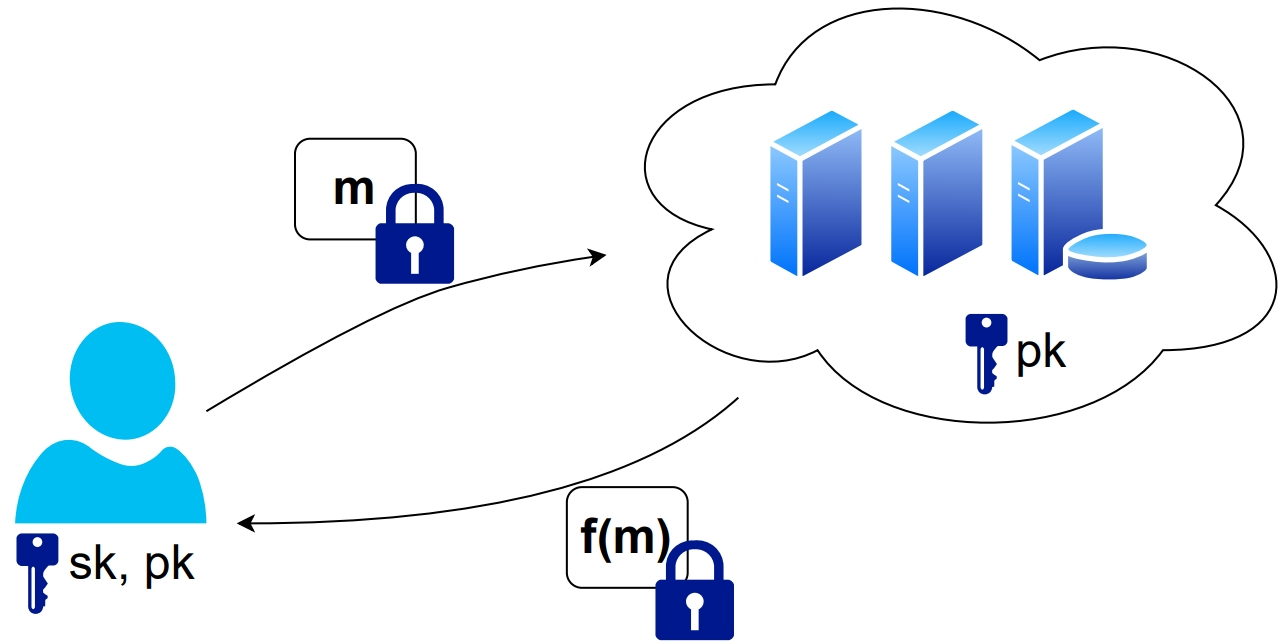
\includegraphics[scale=0.1]{fhe.jpg}
    \caption{Paper:https://ia.cr/2022/657}
\end{figure}
\end{columns}


 \vspace{-0.25cm}
\pause
Ej: Compute a machine learning remotely \textbf{without reveling the data}.
 \vspace{-0.1cm}


Potentially very useful for cloud computing use.
 \vspace{-0.1cm}

 \pause
Present: Orders of magnitude \textbf{slower} for real use.
 \vspace{-0.1cm}

\pause
\begin{mdframed}[backgroundcolor=frenchblue!20]\centering
  Accelerate via hardware.
\end{mdframed}


\end{frame}


%%%%%%%%%%%%%%%%%%%%%%%%%%%%%%%%%%%%%%%%%%%%%%%%%%%%%%%%%%%%%%%%%%%%%%%%%%%%%%%%%%%%%%%%%%%%%%%%%%%%

\begin{frame}
\frametitle{FHE requirements and problems:}
\vspace{0.3cm}
\begin{columns}
    \column{0.6\textwidth}
\begin{itemize}
  \item[\textcolor{frenchblue}{\textbullet}]
Homomorphism in addition and multiplication.
    \begin{itemize}
\pause
      \item[\textcolor{red}{\textbullet}]
Not every scheme is homomorphic in both operations.
    \end{itemize}
\pause
  \item[\textcolor{frenchblue}{\textbullet}]
Unlimited number of operations.
    \begin{itemize}
\pause
      \item[\textcolor{red}{\textbullet}]
Most schemes use \texttt{Learning With Errors} (LWE). Increasing your error for
each operation (mainly in multiplications).
    \end{itemize}
\pause
  \item[\textcolor{frenchblue}{\textbullet}]
Reasonable times.
    \begin{itemize}
\pause
      \item[\textcolor{red}{\textbullet}]
Current schemes have a very large cost for each operation - order of the second.
    \end{itemize}
\end{itemize}
    \column{0.4\textwidth}
\pause
        \begin{figure}[h!]
            \centering
            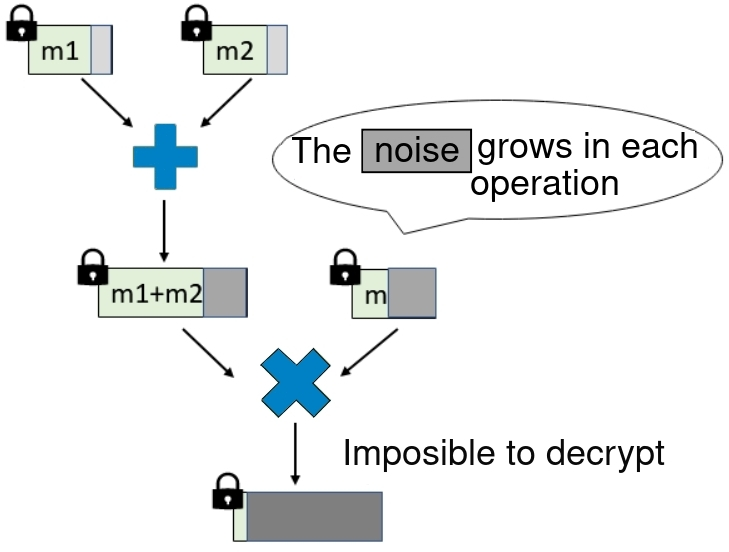
\includegraphics[scale=0.2]{multNoise.jpg}
        \end{figure}

\end{columns}
\pause

Each homomorphic operation is $10^3 \sim 10^6$ times slower than unencrypted.
\pause

Large footprint in memory.
An encrypted date can occupy $10^5$ more space.

\pause
The schemes are iterative, operating many time with each data.
\pause

\begin{mdframed}[backgroundcolor=frenchblue!20]
  Principal bottleneck: technique for reducing error (Bootstrapping)
\end{mdframed}

\end{frame}

%%%%%%%%%%%%%%%%%%%%%%%%%%%%%%%%%%%%%%%%%%%%%%%%%%%%%%%%%%%%%%%%%%%%%%%%%%%%%%%%%%%%%%%%%%%%%%%%%%%%

\begin{frame}
\frametitle{State of art}

FHE is a big topic, with many advances each year.
\vspace{-0.3cm}
\pause

Now a days exists many schemes and some implementations.
\vspace{-0.3cm}
\pause

Schemes:
\begin{itemize}\vspace{-0.3cm}
  \item BFV, BGV: For integers operation.\vspace{-0.3cm}\pause
  \item CKKS: For complex values. Approximate.\vspace{-0.3cm}\pause
  \item FHEW and TFHE:  evaluate arbitrary Boolean circuits on encrypted data.
\end{itemize}
\vspace{-0.3cm}
\pause

        Implementations (open source):
        \begin{itemize}\vspace{-0.3cm}
          \item \textbf{OpenFHE}: designed by (some of)
            the authors of PALISADE, HElib, HEAAN, and FHEW libraries.
            Supports schemes including BGV, BFV, CKKS, TFHE and FHEW,
            written in C++.\vspace{-0.3cm}\pause
          \item \textbf{Microsoft SEAL}: implements BGV and CKKS, written in C++.\vspace{-0.3cm}
          \pause
          \item \textbf{Lattigo}: implements BFV, BGV and CKKS, written in Go.\vspace{-0.3cm}
          \pause
          \item \textbf{Concrete}: implements a variant of TFHE, written in Rust.\vspace{-0.3cm}
        \end{itemize}

\end{frame}


%%%%%%%%%%%%%%%%%%%%%%%%%%%%%%%%%%%%%%%%%%%%%%%%%%%%%%%%%%%%%%%%%%%%%%%%%%%%%%%%%%%%%%%%%%%%%%%%%%%%


\begin{frame}
\frametitle{Starting point}
Scheme: CKKS, more ML appealing for real number operations.
\pause

Framework: OpenFHE, biggest open source community.
\pause

First Tasks:
\begin{itemize}
  \item Get in the math of CKKS.
  \item Compare the math with the implementation.\pause
  \item Profiling: try to detect \texttt{hotpots} to guide us for an efficient
    hardware acceleration and/or software optimization strategy.
\end{itemize}

\end{frame}


%%%%%%%%%%%%%%%%%%%%%%%%%%%%%%%%%%%%%%%%%%%%%%%%%%%%%%%%%%%%%%%%%%%%%%%%%%%%%%%%%%%%%%%%%%%%%%%%%%%%


\begin{frame}
\frametitle{Plans}

Find a particular usage case for FHE to accelerate.
Like:
\begin{itemize}
  \item Autonomous vehicle.
  \item Some ML application: like Ronaks
  \item Search engines: use of private data for adds.
\end{itemize}

\begin{mdframed}[backgroundcolor=frenchblue!20]
  Goal: Accelerate
\end{mdframed}

\end{frame}


%%%%%%%%%%%%%%%%%%%%%%%%%%%%%%%%%%%%%%%%%%%%%%%%%%%%%%%%%%%%%%%%%%%%%%%%%%%%%%%%%%%%%%%%%%%%%%%%%%%%


\end{document}

